  \documentclass[final,letterpaper,oneside,authoryear,11pt,singlespace,spanish]{ezthesis}
\usepackage[spanish]{babel}
\addto\captionsspanish{
\def\bibname{Referencias}
\def\tablename{Tabla}
}
\usepackage{hyperref}
\hypersetup{
    colorlinks=true,
    linkcolor=blue,
    filecolor=blue,      
    urlcolor=blue,
    citecolor=blue
}
\usepackage{rotating}
%%\usepackage{algorithm}
%\usepackage{algpseudocode}
%\usepackage[noend]{algpseudocode}
\usepackage{siunitx}
\usepackage{mathtools}
\usepackage[T1]{fontenc}
\usepackage[utf8]{inputenc}
\usepackage{anysize}
\usepackage{txfonts}
\usepackage{wrapfig} %figura entre texto
\usepackage{times}
\usepackage{listings}
\usepackage{array}
\usepackage{textcomp}
\usepackage{fancyvrb}
\usepackage{fancyhdr}
\usepackage{wallpaper}
\usepackage{verbatim}%Agregado por Luis
\usepackage{latexsym}
\usepackage{url}
\usepackage{multicol}
\usepackage{graphicx}
\usepackage{multirow}
\usepackage{float}
\usepackage{lmodern}
\usepackage{eso-pic}
\usepackage{subfig}
%\usepackage{amssymb}
\usepackage{color}
\usepackage{ragged2e}
\usepackage[all]{xy}
\usepackage{xspace,epic,eepic}
\usepackage{algorithmic}
\usepackage[ruled,vlined]{algorithm2e}
%\usepackage[ruled,vlined,linesnumbered,titlenotnumbered, %portuguese]{algorithm2e}
\usepackage{enumitem}
\setlist{topsep=0pt,noitemsep}
\setcounter{tocdepth}{3}
\marginsize{3cm}{2.5cm}{2.5cm}{2.5cm}

%Definicion de Colores
\definecolor{gray97}{gray}{.97}
\definecolor{gray75}{gray}{.75}
\definecolor{gray45}{gray}{.45}
\definecolor{listinggray}{gray}{0.9}
\definecolor{lbcolor}{rgb}{0.9,0.9,0.9}
\newcommand\rojo[1]{\textcolor[rgb]{1,0,0}{\textbf{#1}}}
\newcommand\red[1]{\textcolor[rgb]{1.00,0.00,0.00}{#1}}
\newcommand\azul[1]{\textcolor[rgb]{0,0,1}{\textbf{#1}}}
\newcommand\blue[1]{\textcolor[rgb]{0,0,1}{{#1}}}
\newcommand\verde[1]{\textcolor[rgb]{0,.5,0.2}{\textbf{#1}}}
\newcommand\naranjo[1]{\textcolor[rgb]{1.00,0.36,0.06}{\textbf{#1}}}
%\ifCLASSINFOpdf
%\else
%\fi
%\hyphenation{pa-la-bra}

\lstset{
	%backgroundcolor=\color{lbcolor},
	tabsize=4,
	rulecolor=,
	language=SQL,
        basicstyle=\small,
        upquote=true,
        aboveskip={1.5\baselineskip},
        columns=fixed,
        showstringspaces=false,
        extendedchars=true,
        breaklines=true,
        prebreak = \raisebox{0ex}[0ex][0ex]{\ensuremath{\hookleftarrow}},
        %frame=single,
        showtabs=false,
        showspaces=false,
        showstringspaces=false,
        identifierstyle=\ttfamily,
        keywordstyle=\color[rgb]{0,0,0},
        commentstyle=\color[rgb]{0,0,0},
        stringstyle=\color[rgb]{0,0,0},
}


%\renewcommand{\labelenumi}{\arabic{enumi}.} % (1., 2., 3.,...)
%\renewcommand{\labelenumi}{\roman{enumi}.} %  (i., ii., iii.,...)
%\renewcommand{\labelenumi}{\Roman{enumi}.} %  (I., II., III.,...)
%\renewcommand{\labelenumi}{\alph{enumi}.}   % (a., b., c.,...)
\renewcommand{\labelenumi}{(\alph{enumi})} % [(a), (b), (c),...]
%\renewcommand{\labelenumi}{\Alph{enumi}.}  %  (A., B., C.,...)


\newtheorem{theorem}{Theorem}[chapter]
\newtheorem{teorema}[theorem]{Teorema}
\newtheorem{lem}{Theorem}[chapter]
\newtheorem{lema}[lem]{Lema}
\newtheorem{prop}{Theorem}[chapter]
\newtheorem{proposition}[prop]{Proposición}
\newtheorem{coro}{Theorem}[chapter]
\newtheorem{corolario}[coro]{Corolario}
\newtheorem{exam}{Theorem}[chapter]
\newtheorem{example}[exam]{Ejemplo}
\newtheorem{test}{Theorem}[chapter]
\newtheorem{prueba}[test]{Prueba}
\newtheorem{defi}{Theorem}[chapter]
\newtheorem{definition}[defi]{Definición}
\newtheorem{obs}{Theorem}[chapter]
\newtheorem{observacion}[obs]{Observación}

\newcommand{\keywords}[1]{\par\addvspace\baselineskip
\noindent\keywordname\enspace\ignorespaces#1}
\renewcommand{\abstractname}{\prefacesection{Resumen}}
%\renewcommand{\tableofcontents}{Índice General}
\renewcommand{\listtablename}{Índice de Tablas}
\renewcommand{\tablename}{Tabla}
\renewcommand{\refname}{Bibliografía}
\newcommand{\boxtheorem}{\hfill $\Box$}
%%%%%%%%IEEE Palabras Claves
%\renewcommand{\IEEEkeywords}{\textbf{\emph{Palabras Clave---}}}


\newcommand{\qed}{\nobreak \ifvmode \relax \else
      \ifdim\lastskip<1.5em \hskip-\lastskip
      \hskip1.5em plus0em minus0.5em \fi \nobreak
      \vrule height0.75em width0.5em depth0.25em\fi}

\author{XXXX XXXX XXXXX}
\title{XXXXX}
\degree{Ingeniería Civil Informática}
\supervisor{XXXX XXXXX XXXXX }
\institution{Universidad del Bío-Bío, Chile}
\faculty{Facultad de Ciencias Empresariales}
\department{Departamento de Sistemas de Información}


\begin{document}
\hyphenation{com-pu-ta-dor}
\cleardoublepage
\pagenumbering{roman}
\setcounter{page}{1}
%% En esta secci'on se describe la estructura del documento de la tesis.
%% Consulta los reglamentos de tu universidad para determinar el orden
%% y la cantidad de secciones que debes de incluir

%% # Portada de la tesis #
%% Mirar el archivo "titlepage.tex" para los detalles.

%% ## Construye tu propia portada ##
%%
%% Una portada se conforma por una secuencia de "Blocks" que incluyen
%% piezas individuales de informaci'on. Un "Block" puede incluir, por
%% ejemplo, el t'itulo del documento, una im'agen (logotipo de la universidad),
%% el nombre del autor, nombre del supervisor, u cualquier otra pieza de
%% informaci'on.
%%
%% Cada "Block" aparece centrado horizontalmente en la p'agina y,
%% verticalmente, todos los "Blocks" se distruyen de manera uniforme
%% a lo largo de p'agina.
%%
%% Nota tambi'en que, dentro de un mismo "Block" se pueden cortar
%% lineas usando el comando \\
%%
%% El tama'no del texto dentro de un "Block" se puede modificar usando uno de
%% los comandos:
%%   \small      \LARGE
%%   \large      \huge
%%   \Large      \Huge
%%
%% Y el tipo de letra se puede modificar usando:
%%   \bfseries - negritas
%%   \itshape  - it'alicas
%%   \scshape  - small caps
%%   \slshape  - slanted
%%   \sffamily - sans serif
%%
%% Para producir plantillas generales, la informaci'on que ha sido inclu'ida
%% en el archivo principal "tesis.tex" se puede accesar aqu'i usando:
%%   \insertauthor
%%   \inserttitle
%%   \insertsupervisor
%%   \insertinstitution
%%   \insertdegree
%%   \insertfaculty
%%   \insertdepartment
%%   \insertsubmitdate
\begin{titlepage}
  \TitleBlock{
\includegraphics[height=3cm]{figures/UBB.png}}
  \TitleBlock{\scshape\insertinstitution}
  \TitleBlock[\bigskip]{\scshape\insertfaculty}
  \TitleBlock[\bigskip]{\insertdepartment}
  \TitleBlock{\Huge\scshape\inserttitle}
  \TitleBlock{\scshape
    Anteproyecto de título presentado por\\
     \insertauthor \\
    de la Carrera \insertdegree\\
    Dirigida por \\
    \insertsupervisor}
  \TitleBlock{\insertsubmitdate}

\end{titlepage}



%% # Prefacios #
%% Por cada prefacio (p.e. agradecimientos, resumen, etc.) crear
%% un nuevo archivo e incluirlo aqu'i
%% Para m'as detalles y un ejemplo mirar el archivo "gracias.tex".

%
\chapter*{Resumen\markboth{Resumen}{Resumen}}

\renewcommand{\keywords}{\textbf{\emph{Palabras Clave ---~}}}

Debe describir su proyecto, resultados y beneficios esperados.



\keywords{xxxx,xxxxx,xxxxx} 


\chapter*{Resumen\markboth{Resumen}{Resumen}}

\renewcommand{\keywords}{\textbf{\emph{Palabras Clave ---~}}}

Debe describir su proyecto, resultados y beneficios esperados.



\keywords{xxxx,xxxxx,xxxxx} 


\chapter*{Dedicatoria y/o Agradecimientos\markboth{Dedicatoria}{Dedicatoria}}


Debe describir su proyecto, resultados y beneficios esperados.






\chapter*{Acronimos\markboth{Acronimos}{Acronimos}}







%\renewcommand{\tableofcontents}{Índice General}
%\tableofcontents
\renewcommand\contentsname{Índice General}
\tableofcontents


%\listoffigures
\renewcommand{\listfigurename}{Índice de Figuras}
\listoffigures


\renewcommand{\listtablename}{Índice de Tablas}
\listoftables

\cleardoublepage
\pagenumbering{arabic}
\setcounter{page}{1}

\chapter{Introducción}
\label{cap:introduccion}
Introducción al tema




\section{Descripción del Problema}

Describir el problema


\subsection{Descripción de la Organización y Área de trabajo}

En el texto responda a las preguntas: para que empresa/institución, quienes son, donde se ubican, desde cuándo, que hacen u ofrecen, quienes son sus clientes. 
En qué ámbito de la empresa/institución se enmarca este proyecto.

\subsection{Proceso de Negocio Actual}

Explique la situación actual a través de una descripción de los procesos o actividades que han dado origen a este proyecto. 

\subsection{Explicación del proceso de negocio}

Utilice cualquier tipo de diagrama, por ejemplo, 
diagrama de procesos de negocios (notación BPMN), o 
diagrama de actividad (UML 2.0) o 
diagrama de procedimiento adm.
 
Recuerde referenciar la figura en un texto como por EJEMPLO 

“A continuación, la Figura 1 representa los procedimientos que se siguen actualmente en la empresa.” Debe explicar el modelo, tal como “leer el modelo” sin entrar en detalles innecesarios. 
Incluya título para la figura, por ejemplo “Figura 1: Diagrama de Actividad, notación UML2.0 para representar el procedimiento para …..”.

\section{Definición de usuarios}
\subsection{Caracterización de los usuarios}
\subsection{Problemas de información de los usuarios}

\subsection{Oportunidades de Mejora o Problemáticas}

Se identifica y especifica el problema o la oportunidad de mejora que ha motivado la necesidad del sistema, lo cual definirá el objetivo del sistema. NO SE COMENTA LA SOLUCIÓN.

\subsection{Propuesta de solución}

Debe explicar en términos generales cómo las TIC pueden resolver o mejorar la(s) problemática identificada y quienes serán los usuarios principales, que tecnología se utilizaría para dar soporte a la propuesta. 

\section{Soluciones Similares disponibles}

Se investigó en biblioteca Werken, en el buscador de Google, Play Store y en App Store con fecha xxxxxxxxxxxxxx con el propósito de conocer que otras soluciones existen actualmente. 


\section{Justificación del Proyecto}

Comente las razones técnicas, económicas, funcionales, sociales etc por las que ESTE PROYECTO ES importante que sea desarrollado.
Esto generalmente se escribe inicialmente en la propuesta del tema.


\section{Objetivos del proyecto}
\subsection{Objetivo general}

Objetivos generales del proyecto, estos objetivos son distintos a los objetivos del software/sistema de Sw. Utilice sólo1 verbo activo por objetivo
Los Objetivos del proyecto terminan con el proyecto y los objetivos del software se logran con el uso del software, es decir van más allá de la fecha de término del proyecto. 
Por ejemplo, un objetivo del proyecto puede comenzar como “implementar una solución a…”


\subsection{Objetivos específicos}

Utilice sólo1 verbo activo por objetivo, No confunda los objetivos con las actividades que serán desarrolladas, la lógica o relación es que los objetivos son metas, se pueden ser alcanzables una vez terminadas varias actividades.
hacer entrevistas, cuestionarios
Revisar información 
Evaluar procesos
proponer la solución Sw obj

\subsection{Actividades para Realización del Proyecto}

En la siguiente sección se describe la actividades a realizar para la investigación, por objetivos específicos.
\begin{itemize}
    \item 
    \item 
    \item 
    \item 
    \item 
    \item 
    
\end{itemize}



\section{Composición del Informe} 

El presente trabajo se encuentra dividido en xx capítulos. A continuación se describe brevemente el contenido de cada uno de ellos.

no usar viñetas, solo párrafos....\\




\chapter{Análisis} 
\label{cap:analisis}

El presente capítulo tiene por objetivo describir los principales conceptos asociados a la formación de complejos proteicos y a su predicción, facilitando al lector la comprensión de las secciones posteriores.


\section{Ambiente de Desarrollo de Ingeniería de Software}
\subsection{Metodología de Desarrollo}

La metodología de desarrollo a utilizar en el proyecto es ... 
Esta metodología fue seleccionada ya que este proyecto ...
este software ...

\subsection{Tecnologías Utilizadas (Backend, Frontend, Base de Datos)}



\subsection{Estándares de Documentación}

Adaptación basada en IEEE Software Test Documentation Std 829-1998 
Adaptación basada en IEEE Software Requirements Specifications Std 830-1998

\subsection{Técnicas y notaciones}

ejemplo: Diagramas de Casos de Uso -notación UML es utilizada para detallar la funcionalidad del software 

\subsection{Herramientas, framework, lenguaje usados en el desarrollo del proyecto}

ejemplo: MongoDBCompass versión 1.33.0, herramienta utilizada para la consulta de las estructuras de datos -collections

\section{Especificación de requerimientos - Producto SW}
\subsection{Límites}

El software / app no permitirá ...

\subsection{Rectricciones Técnicas}

La empresa cuenta con ...

\subsection{Objetivo General y Especificos de SW}

\subsubsection{Objetivo General}

Defina sólo 1 objetivo general. Utilice 1 verbo activo que englobe la contribución o aporte del software completo en la empresa. Todos los objetivos de software se escriben así: El sistema HACE ALGO con lo que la empresa REDUCE COSTOS/ AUMENTA  INGRESOS/ AUMENTA UTILIDAD 
Por ejemplo: El sistema manejará información del proceso de postulación de a cargos para que la empresa optimice el uso de los recursos utilizados en el proceso, es decir reduciendo los recursos gastados por todos los involucrados en el registro, evaluación y resultados.

\subsubsection{Objetivos Especificos de SW}

Utilice 1 verbo activo que contribuya al objetivo general, es decir la contribución de ciertas funciones del software en la empresa. Todos los objetivos de software se escriben así: El sistema HACE ALGO con lo que la empresa REDUCE COSTOS/ AUMENTA  INGRESOS/ AUMENTA UTILIDAD. Por Ejemplo: 
\begin{itemize}
    \item El sistema permite que los postulantes sean notificados directamente, se mantengan todos informados de las etapas y actividades a realizar, de esta forma la empresa elimina el tiempo de la secretaria en confirmaciones telefónicas o agenda de entrevistas.
    \item El sistema permite que las postulaciones sean realizadas por los postulantes y solo aquellas que cumplen con los requisitos obligatorios sean revisadas por el comité, de esta forma la empresa elimina el tiempo de la secretaria y de la comisión revisando curriculum incompletos.
\end{itemize}

\subsection{Planificación de reuniones con usuarios}
\subsection{Requerimientos Funcionales}

La lista de los requerimientos funcionales específicos se presenta en la Tabla 10.
• Los \begin{itemize}
    \item requerimientos pueden ser agrupados por distintos criterios, por ejemplo, tipo de usuario o módulo (otras organizaciones se encuentran en el anexo del estándar IEEE Std 830-1998).
    \item Se recomienda el uso de la forma verbal en infinitivo para denotar las acciones que el software debe realizar.
    \item Los requerimientos deben ser enumerados para facilitar su seguimiento. 
    \item En la descripción de cada requerimiento se incluyen condiciones o restricciones del requerimiento, por ejemplo “los registros de los clientes pueden ser eliminados si y sólo si el cliente no ha efectuado ninguna compra en los 5 últimos años”. 
    \item Los requerimientos de su proyecto considerando se redactan contestando, al menos, las preguntas: Quien, Que, Que restricciones existen, Cuando, Que pasa después? Por ejemplo: 
    
    El CLIENTE o la ENCARGADA de recepción pueden REGISTRAR reserva de habitaciones, el cliente NO REQUIERE estar registrado y puede reservar COMO MÁXIMO 10 habitaciones a través de la web. La encargada de recepción puede reservar MÁS DE 10 habitaciones con la autorización del Encargado de Administración. Se puede registrar reserva SÓLO SI EXISTE DISPONIBILIDAD en fecha y habitaciones. El registro EXITOSO genera un código de reserva, y la reserva que queda en estado no confirmada.
    \item Sino se especifican los requisitos contestando a las preguntas no será evaluado
\end{itemize} 

 \begin{table}[H]
    \begin{center}
        \begin{tabular}{ | m{2cm} | m{9cm} | }
            \hline \textbf{id} & \textbf{el sistema debe }\\ \hline
            RF\_01 &   \\ \hline
            RF\_02 &     \\ \hline
              &    \\ \hline
        \end{tabular}
        \caption{Requerimientos Funcionales}
    \end{center}
\end{table}

\subsection{Requerimientos No Funcionales}

Misma idea de arriba

\subsection{Interfaces externas de Entrada}

Cada interfaz externa, es una especificación tomada desde IEEE Std 830-1998 página 22, tal como lo muestra la figura. Se separa en ENTRADA Y SALIDA.

\begin{figure}[H]
    \centering
    
\includegraphics[scale=0.5]{figures/i1.png}
    \caption{Ejemplo1}
    \label{fig:e1}
\end{figure}

\begin{figure}[H]
    \centering
    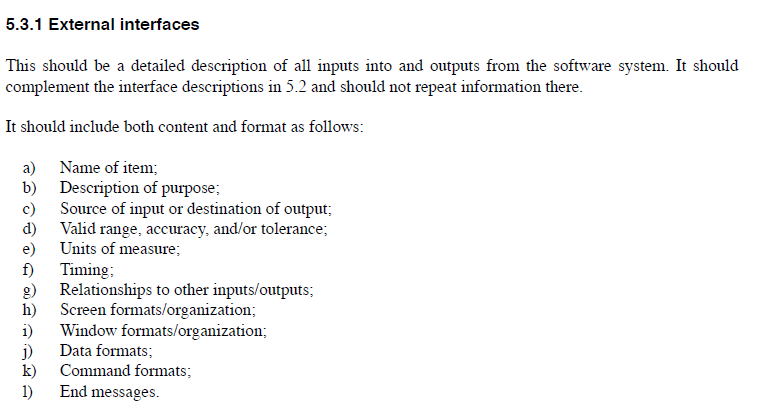
\includegraphics[scale=0.5]{figures/i2.png}
    \caption{Ejemplo2}
    \label{fig:e2}
\end{figure}

Interfaz externa de entrada, es decir un conjunto de datos que serán ingresados al sistema independiente del medio de ingreso, es decir datos que provienen de un usuario a través de teclado, lector de código barra, etc.
En la tabla se incluyen los ítems de datos 1 sola vez, por ejemplo, no es necesario repetir el rut del proveedor o el código del producto, en esta tabla importan QUE DATOS INGRESARÁN y no importa cuántas veces ingresen.

 \begin{table}[H]
    \begin{center}
        \begin{tabular}{ | m{2cm} | m{3cm} | m{9cm} |}
            \hline \textbf{Identificador} & \textbf{Nombre del ítem} & \textbf{Detalle de Datos contenidos en ítem} \\ \hline
            Ejemplo: 
            DE\_01 & Datos del proveedor  & NOMBRE, RUT\_PROV, GIRO, DIRECCION,TELEFONO ...\\ \hline
            DE\_02 & Datos de factura & RUT\_PROV,FECHA\_FACT, TIPO\_PAGO, COD\_PROD, CANT\_COMPRADA, PRECIO …….   \\ \hline
            DE\_03 & Datos de productos & COD\_PROD, NOMBRE   \\ \hline
                  &        & \\ \hline
        \end{tabular}
        \caption{Interfaces de Entrada}
    \end{center}
\end{table}

\subsection{Interfaces externas de Salida}

Se especifica cada salida del sistema, conjuntos de datos que se sacan del sistema para los usuarios u otros sistema,  indicando en cada caso el formato o medio de salida. 


 \begin{table}[H]
    \begin{center}
        \begin{tabular}{ | m{2cm} | m{3cm} | m{8cm} | m{2cm} |}
            \hline \textbf{Identificador} & \textbf{Nombre del ítem} & \textbf{Detalle de Datos contenidos en ítem} & \textbf{Medio Salida}\\ \hline
            Ejemplo: 
            IS\_01 & Informe de los proveedores  & NOMBRE, RUT, CODIGO,GIRO,DIRECCION,TELEFONO & Archivo XLS, Impresora, Pantalla\\ \hline
             &  &  & \\ \hline
             &  &  & \\ \hline
             &  &  & \\ \hline
        \end{tabular}
        \caption{Interfaces de Salida}
    \end{center}
\end{table}

\section{Factibilidad del Proyecto}
\subsection{Factibilidad Técnica}

Describa si:
\begin{itemize}
    \item Existen las personas para construir el software, si las personas tienen los conocimientos y competencias técnicas.
    \item Existen o se pueden adquirir sw de desarrollo y necesario para explotación del sw
    \item Existen o se pueden adquirir Hw de desarrollo (pc y server) y necesario para explotación del sw (server)
\end{itemize}




 \begin{table}[H]
    \begin{center}
        \begin{tabular}{ | m{5cm} | m{6cm} | }
            \hline \textbf{REQUERIMIENTOS} & \textbf{DESCRIPCIÓN }\\ \hline
            Sistema operativo   & Ubuntu 20.04 o superior. \\ \hline
            Procesador          & Pentium silver. \\ \hline
            Memoria RAM         & 4 GB. \\  \hline
            Espacio de almacenamiento & 2 GB.\\\hline
            Navegador           & safari, Opera, etc.\\ \hline
            Resolución de pantalla &  1280 x 768 px.\\ \hline
            Conexión a internet & Requerida.\\ \hline
        \end{tabular}
        \caption{Especificación de Software requerido en desarrollo del proyecto}
    \end{center}
\end{table}


 \begin{table}[H]
    \begin{center}
        \begin{tabular}{ | m{5cm} | m{6cm} | }
            \hline \textbf{REQUERIMIENTOS} & \textbf{DESCRIPCIÓN }\\ \hline
            XX & XX  \\ \hline
            XX & XX  \\ \hline
        \end{tabular}
        \caption{Especificación de Hardware requerido en desarrollo del proyecto}
    \end{center}
\end{table}


 \begin{table}[H]
    \begin{center}
        \begin{tabular}{ | m{5cm} | m{6cm} | }
            \hline \textbf{REQUERIMIENTOS} & \textbf{DESCRIPCIÓN }\\ \hline
            XX & XX  \\ \hline
            XX & XX  \\ \hline
        \end{tabular}
        \caption{Especificación de Hardware Servidor requerido en desarrollo del proyecto}
    \end{center}
\end{table}


Concluya si todo existe o se puede adquirir, o hay una comunidad de apoyo ... es técnicamente factible.


\subsection{Factibilidad Operativa}

Describa si:
\begin{itemize}
    \item Los clientes reconocen la importancia del sw y sus beneficios.
    \item Los usuarios reconocen la importancia del sw y sus beneficios.
    \item Los usuarios están disponibles a participar, tienen las competencias mínimas requeridas
\end{itemize}
Si lo anterior existe, o usted tomará las medidas para reforzarlo, entonces es operativamente factible.


\subsection{Factibilidad Económica}
Describa:

 \begin{table}[H]
    \begin{center}
        \begin{tabular}{ |l|l|l| }
            \hline 
            \textbf{Software} & \textbf{Licencia} & \textbf{Costo Licencia}\\ \hline
            XX & XX & XX  \\ \hline
            XX & XX & XX \\ \hline
        \end{tabular}
        \caption{Licencias}
    \end{center}
\end{table}

 \begin{table}[H]
    \begin{center}
        \begin{tabular}{ |l|l|l| }
            \hline 
            \textbf{Item} & \textbf{\$ mensual aprox. en CLP} & \textbf{\$ anual aprox. en CLP}\\ \hline
            XX & XX & XX  \\ \hline
            XX & XX & XX \\ \hline
        \end{tabular}
        \caption{Costo hosting y dominio, Este servicio tiene un costo anual obtenido de https://www.nic.cl/dominios/tarifas.html}
    \end{center}
\end{table}

\begin{table}[H]
    \begin{center}
        \begin{tabular}{ |m{2cm}|m{2cm}|m{5cm}|m{5cm}| }
            \hline 
            \textbf{Recurso Humanos} & \textbf{Cantidad personal} & \textbf{Sueldo aprox. en CLP por mes} &
            \textbf{Sueldo aprox. en CLP por duración proyecto (x meses)}\\ \hline
            XX & XX & XX & XX \\ \hline
            XX & XX & XX & XX\\ \hline
        \end{tabular}
        \caption{ Calculo costo de desarrollo y soporte.}
    \end{center}
\end{table}

\subsubsection{Flujo de caja}

Para asegurar la viabilidad económica del proyecto, se empleará el indicador del Valor Actual Neto (VAN) como medida. Para ello, se realizará el cálculo del flujo de caja correspondiente a la inversión inicial, así como se proyectarán los flujos de caja para los primeros 5 años. Estos datos se presentan en detalle en la siguiente tabla:

\begin{table}[H]
    \begin{center}
        \begin{tabular}{ |m{2cm}|m{2cm}|m{1cm}|m{1cm}|m{1cm}|m{1cm}|m{1cm}| }
            \hline 
            \textbf{Recurso Humanos} & \textbf{Año 0} & \textbf{Año 1} &
            \textbf{Año 2} & \textbf{Año 3} & \textbf{Año 4} & \textbf{Año 5} \\ \hline
            (+) Ingresos &  &  &  &  &  & \\ \hline
            Beneficios   & \$ costo desarrollo (ahorro) \$ reducción de costos
            (ahorro) & XX & XX & XX & XX & XX\\ \hline
            (-) Costos   &  &  &  &  &  & \\ \hline
            &  &  &  &  &  &\\ \hline
            Servicios & (\$b) & (\$b) & (\$b) & (\$b) & (\$b) & (\$b)\\ \hline
            Soporte y Mantención & (\$a) & (\$a) & (\$a) & (\$a) & (\$a) & (\$a)\\ \hline
            TOTAL & (\$ab) & (\$ab) & (\$ab) & (\$ab) & (\$ab) & (\$ab)\\ \hline
        \end{tabular}
        \caption{ Calculo costo de desarrollo y soporte.}
    \end{center}
\end{table}


\subsubsection{Cálculo del V.A.N}

Donde cada uno de los términos, se especifican en la Tabla:


 \begin{table}[H]
    \begin{center}
        \begin{tabular}{ | m{2cm} | m{8cm} | }
            \hline \textbf{Término} & \textbf{Significado }\\ \hline
            $t$ & Intervalo de tiempo   \\ \hline
            $n$ & Duración en años  \\ \hline
            $I_0$ & Inversión inicial $(t=0)$   \\ \hline
            $K$ & Tasa de descuento   \\ \hline
            $Vt$ & Flujos de caja obtenidos en el intervalo de tiempo $t$   \\ \hline
        \end{tabular}
        \caption{Términos de la fórmula de VAN}
    \end{center}
\end{table}

A continuación, se calculará el VAN con una tasa de descuento del 10%.

 \begin{table}[H]
    \begin{center}
        \begin{tabular}{ | m{5cm} | m{6cm} | }
            \hline \textbf{Año} & \textbf{Flujo de Caja }\\ \hline
            \textbf{Año 0} & $\$ab/(1+0.10)^0 = \$$  \\ \hline
            \textbf{Año 1} & $\$ab/(1+0.10)^1 = \$$  \\ \hline
            \textbf{Año 2} & $\$ab/(1+0.10)^2 = \$$  \\ \hline
            \textbf{Año 3} & $\$ab/(1+0.10)^3 = \$$  \\ \hline
            \textbf{Año 4} & $\$ab/(1+0.10)^4 = \$$  \\ \hline
            \textbf{Año 5} & $\$ab/(1+0.10)^5 = \$$  \\ \hline
        \end{tabular}
        \caption{Cálculo del VAN}
    \end{center}
\end{table}

$ VAN (10\%) = Año 0 + Año 1 + Año 2 + Año 3 + Año 4 + Año 5 $

$             = \$ $

$ VAN (10\%) = \$ $


En este caso, el VAN obtenido es positivo (\$   ), lo que indica que el proyecto es viable desde una perspectiva económica.

\subsection{Conclusión de Factibilidad}

Gracias al análisis realizado en los puntos anteriores, se puede concluir que el proyecto es 


\chapter{Diseño} 
\label{cap:disenno}

Introducción al capítulo

\section{Descripción de los servicios web - necesarios}
\section{Modelo de datos}

Debe explicar el modelo de datos, relacional o no-relacional, es decir leerlo destacando las entidades, colecciones y/o relaciones -referencias fundamentales en la problemática.
Diagrama con Modelo de datos relacional o no relacional

\begin{figure}[H]
    \centering
    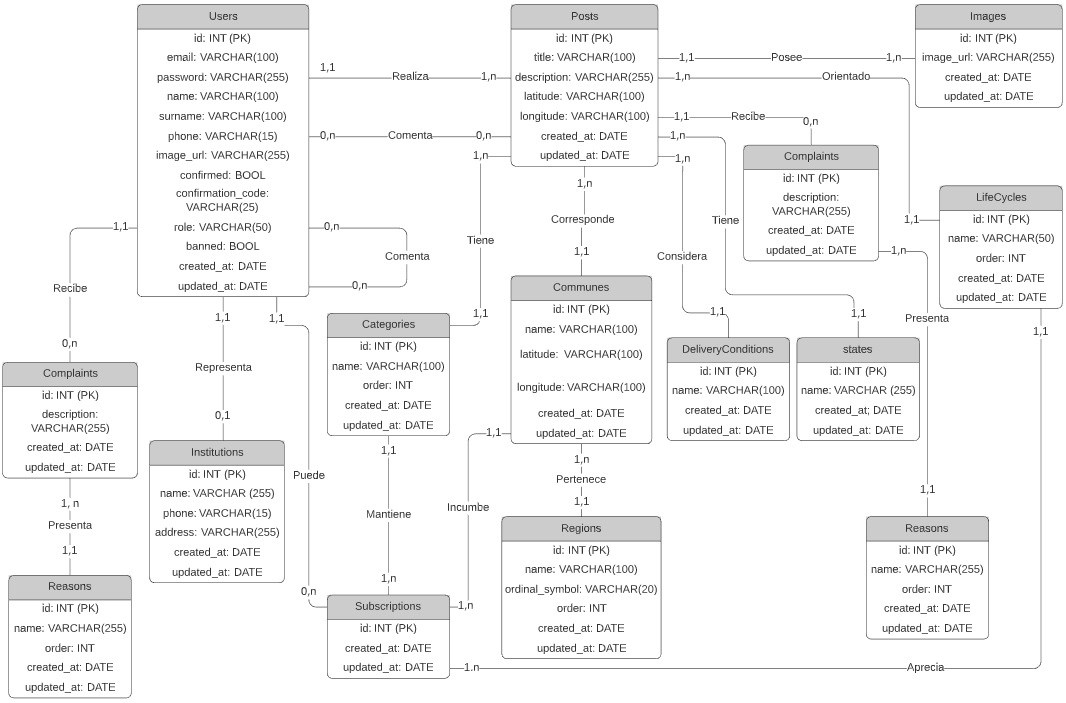
\includegraphics[scale=0.5]{figures/i4.jpg}
    \caption{XX}
    \label{fig:i4}
\end{figure}

\begin{figure}[H]
    \centering
    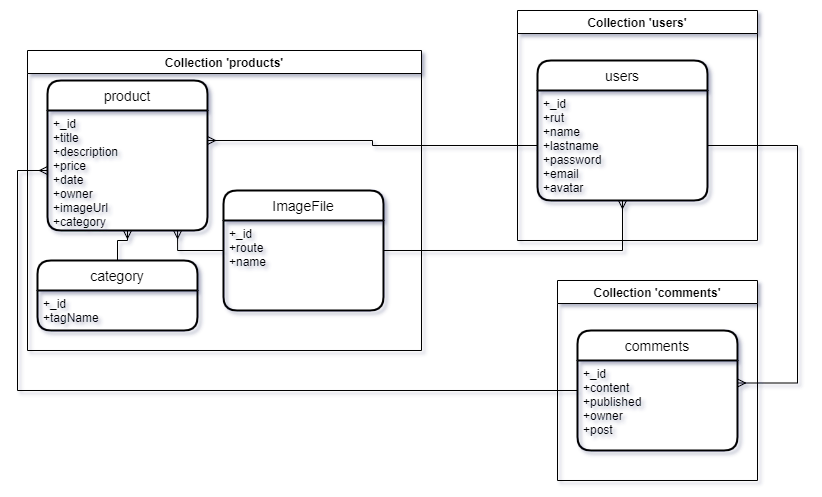
\includegraphics[scale=0.5]{figures/i5.png}
    \caption{xx}
    \label{fig:i5}
\end{figure}

\subsection{Esquema de la base de datos}

A continuación, se describen los datos y tipos de la BD, en formato JSON.

Esquema products : 

% Se dejo en comentarios, porque depende de lo que hagan
%{
%    title: {
%        type: String,
%        required: true
%    },
%    description: {
%        type: String,
%        default: null
%    },
%    price: {
%        type: Number,
%        required: true
%    },
%    date: {
%        type: Date,
%        required: true
%    },
%    imageUrl: [{
%        type: Schema.ObjectId,
%        ref: "imageFile"
%    }],
%    owner: {
%        type: Schema.ObjectId,
%        ref: "user"
%    },
%    category: [{
%        type: Schema.ObjectId,
%        ref: "category"
%    }],
%}

\subsection{Entidad-Relación}
\subsection{Modelo Relacional}


\section{Casos de uso (o Historias de usuario)}
\subsection{Actores de casos de uso}

Los actores que interactúan con el sistema se detallan en la Tabla 13.

\begin{table}[H]
    \begin{center}
        \begin{tabular}{ |m{2cm}|m{2cm}|m{3cm}|m{3cm}|m{3cm}| }
            \hline 
            \textbf{Actor} & \textbf{Cargo(s)} & \textbf{Funciones en la empresa} &
            \textbf{Nivel de conocimeintos técnicos requeridos} & \textbf{Nivel privilegio en el sistema} \\ \hline
              &   &   &   &  \\ \hline
              &   &   &   &  \\ \hline
        \end{tabular}
        \caption{ Calculo costo de desarrollo y soporte.}
    \end{center}
\end{table}

En el caso de que existen generalizaciones de actores incluya los diagramas correspondientes.

\subsection{Diagramas}

Incluya más de 1 diagrama para que quede claro el modelo.
Diagrama(s) de CU


\begin{figure}[H]
    \centering
    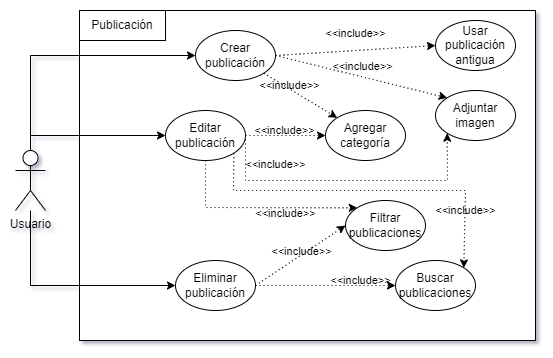
\includegraphics[scale=0.5]{figures/i3.png}
    \caption{Diagrama de Casos de Uso publicaciones – ejemplo tesis Tomás Montecinos IECI}
    \label{fig:e3}
\end{figure}

\subsection{Especificación de casos de uso}

Liste los CU que están en su (s) diagramas destacando cuales serán detallados.
Considerando funcionalidad RELEVANTE del negocio especifique con la tabla sólo los CU relacionados. Para los CU restantes sólo incluya una descripción y precondiciones.


\begin{figure}[H]
    \centering
    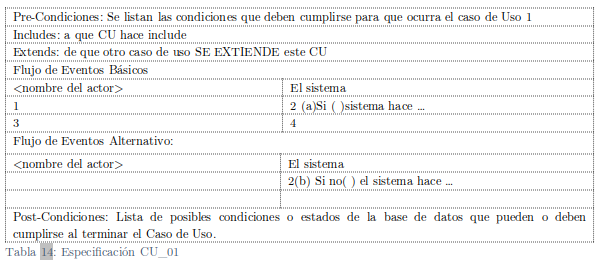
\includegraphics[scale=0.5]{figures/i12.png}
    \caption{E1}
    \label{fig:i12}
\end{figure}

Ejemplos:

\begin{figure}[H]
    \centering
    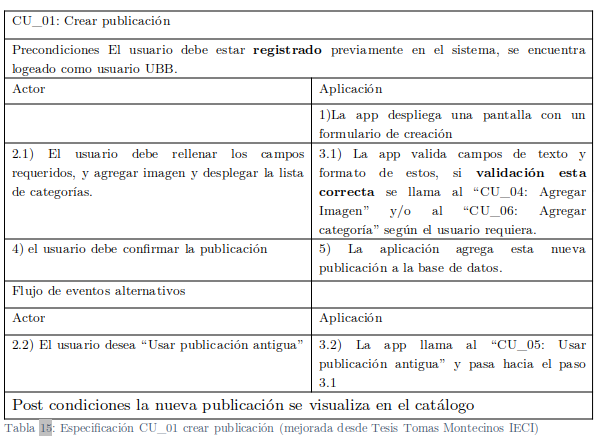
\includegraphics[scale=0.5]{figures/i13.png}
    \caption{E2}
    \label{fig:i13}
\end{figure}



\section{Diseño de interfaz y navegación (Mockups)}

\subsection{Guías de estilos}

La guía de estilo marcará las pautas a seguir para el diseño de la web. Por tanto, servirá
de consulta para visualizar los objetivos de la aplicación en cuanto a su estilo. El principal
objetivo es dotar al estilo de la aplicación de la máxima sencillez posible, a fin de que al
usuario le resulte intuitivo el uso de la aplicación.
A continuación se señalarán aspectos relativos al estilo como son el logotipo, los colores
principales y secundarios, la tipografía y la composición de las interfaces.
\subsubsection{Logotipo}
El logotipo es el símbolo que representa la temática de la aplicación. Esta imagen podrá ser presentada de diferentes formas, como son el imagotipo y el isotipo. Además, se mostrarán dos versiones de cada representación: una en color y otra en blanco y negro.
Por lo que respecta al isotipo, en la figura 8.8, este se caracteriza por no tener ningún texto. El icono representativo se caracteriza por estar compuesto por dos elementos. El principal es un coche con 5 pasajeros, simbolizando el hecho de compartir coche, mientras que el secundario se trata del icono representativo de la ubicación con un birrete, que simboliza el hecho de encontrar estudiantes.

\begin{figure}[H]
    \centering
    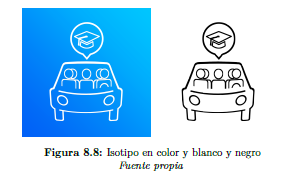
\includegraphics[scale=0.5]{figures/i11.png}
    \caption{autitos}
    \label{fig:i11}
\end{figure}

\subsection{Guía de colores}

Los colores corporativos de la aplicación componen una gama cromática fría, orientada a
tonos azules. En primer lugar, los colores corporativos que se utilizarán mayoritariamente en el diseño de las interfaces están reunidos en la paleta de la figura 8.10. Por una parte, “Bluetiful” y “Vivid Sky Blue” serán los colores de los elementos con los que el usuario podrá interactuar, como botones y enlaces. Y, por otra parte, “Black Chocolate” y “Azyre X Web Color” serán los correspondientes al texto y fondo de la aplicación

\begin{figure}[H]
    \centering
    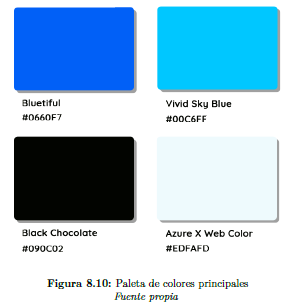
\includegraphics[scale=0.5]{figures/i9.png}
    \caption{autitos}
    \label{fig:i9}
\end{figure}

No obstante, a estos colores principales se les añadirán 3 más que estarán relacionados con la acción que realizan los botones en los que se apliquen. Se trata del color “Rufous” para acciones como “Eliminar” y “Cancelar”, el “Maximum Yellow” para “Editar” y “Leaf Green” para “Enviar” y “Aceptar”.

\begin{figure}[H]
    \centering
    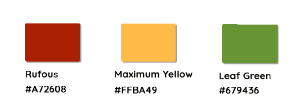
\includegraphics[scale=0.5]{figures/i8.png}
    \caption{autitos}
    \label{fig:i8}
\end{figure}

\subsubsection{Tipografía}

La tipografía utilizada es un tipo de letra sencilla y universal que facilite la legibilidad. Se ha optado por emplear una fuente gratuita de Google Fonts, como es Roboto. En la figura se incluye una representación de dicha fuente con los caracteres más comunes.

\begin{figure}[H]
    \centering
    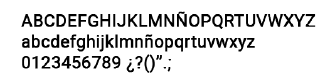
\includegraphics[scale=0.5]{figures/i10.png}
    \caption{autitos}
    \label{fig:i10}
\end{figure}

\subsection{Composición de las interfaces}

La composición de las interfaces expuesta a continuación corresponde a la versión adaptada para móvil, que será la versión implementada en primer lugar. La adaptación para pantallas de mayor tamaño se realizará en un futuro.
Distinguiremos entre 3 tipos de interfaces según su composición: lista, tarjeta y formulario. La comparación entre ellas puede observarse en la figura 

\begin{figure}[H]
    \centering
    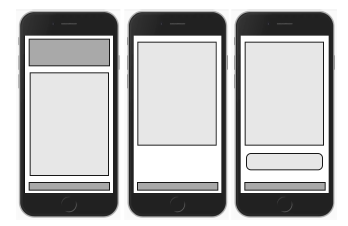
\includegraphics[scale=0.5]{figures/i7.png}
    \caption{autitos}
    \label{fig:i7}
\end{figure}

<Incluye al menos 3 mockups o screenshot de las interfaces propuestas que representan el estándar que será seguido en el sw>.

Recuerde: El diseño de la interfaz de usuario debe considerar un diseño estándar que será respetado en todas las pantallas. En el diseño se considera la organización y el aspecto de la interfaz. El aspecto considera muchos elementos, entre ellos, los colores, imágenes de fondo, uso de iconos entre otros. La organización de una pantalla considera la ubicación de cada uno de los tipos de elementos de la interfaz, considerando por ejemplo las siguientes áreas:  De ingresos de datos, De Botones de opción general, De botones de opciones específicas a la ventana, De Menús, De títulos,  De Barras de Herramientas, De pie de página, De Encabezados, y De Logos


\chapter{Desarrollo del Trabajo} 
\label{cap:desarrollo}

Aqui el alumno debe describir su proceso de trabajo, como se trabajo, problemas, lo que funciono, pruebas de tecnologias ...

\section{Diseño de arquitectura}

Especificar la decisión relacionada respecto a servidores de datos y aplicación (web)
\begin{itemize}
    \item Servidores propios,
    \item Hosting, 
    \item Cloud, otros o mezcla de ellos.
\end{itemize}
Incluya un esquema que represente la integración de estos elementos, desde el punto de vista físico y lógico. Este diagrama debe ser explicado. Por ejemplo: 
Tal como se representa en la Ilustración 2 la arq. que da soporte al  sw “mi software” se divide en 2 servidores físicos, ATLANTA y MARCUS. 
EL primero aloja el server web sobre un SO apache xxx, para el sw mio.midominio.cl http://146.83.99.99, puerto ssh 999 u puerto apache 999. El segundo  servidor físico aloja 2 componentes lógicos, servidor de archivos user/carpeta/ y de base de datos con Mysql 192.168.l.0 (ejemplo). Los usuarios locales acceden a través de los sistemas distribuidos por red local y al sistema web vía internet…. etc.
El escenario es distinto si se trabaja con contenedores, si se utilizan servicios web, API, o la nube amazon ws, azure, etc

\begin{figure}[H]
    \centering
    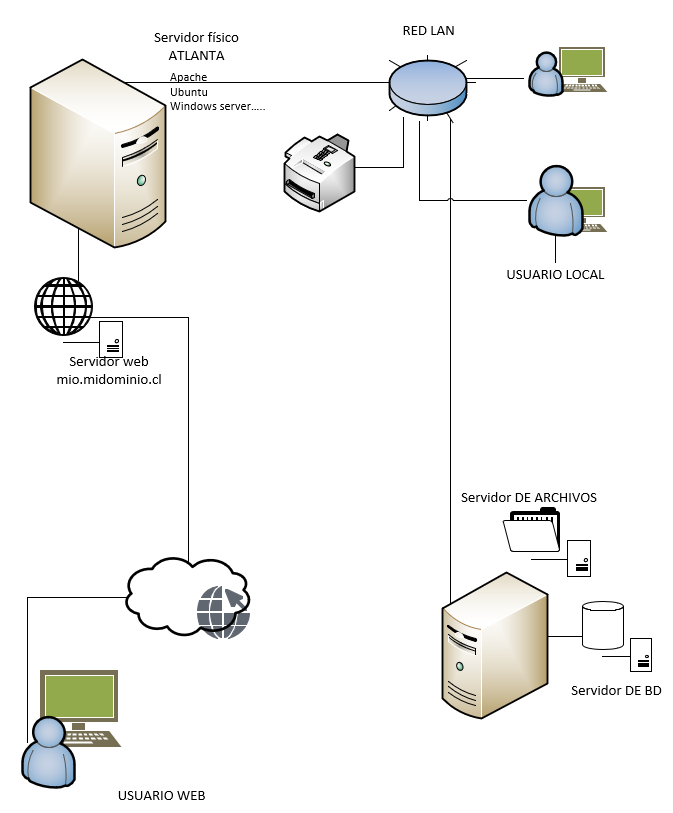
\includegraphics[scale=0.5]{figures/i6.png}
    \caption{Ejemplo2}
    \label{fig:e6}
\end{figure}


\section{Estructura del código}

Si se utiliza framework o se programa en lenguaje web puro indicar la forma como se organizan físicamente los archivos y si estos respetan alguna arquitectura de programación como modelo vista controlador, o 3 capas, etc. Incluya una imagen del árbol de directorio.

\subsection{Backend}

 \begin{table}[H]
    \begin{center}
        \begin{tabular}{ | m{2cm} | m{8cm} | }
            \hline \textbf{Directorio} & \textbf{Detalle }\\ \hline
            Controllers & Funciones con las que cuenta la aplicación al momento de comunicarse con el servidor de base de datos y viceversa.   \\ \hline
                &    \\ \hline    
                &    \\ \hline   
              \end{tabular}
        \caption{E2}
    \end{center}
\end{table}


Funcionalidad- Endpoints a utilizar:
\begin{enumerate}
    \item 1. http://”URLPROYECTO”.cl/”RUTA A UTILIZAR”
    \begin{enumerate}
        \item a. Tipo de petición:
            \begin{itemize}
               \item i. “get,post,put,delete”
            \end{itemize}
        \item b. Parámetros a ingresar, el tipo de datos y restricciones
            \begin{enumerate}
                \item i. Nombre
                    \begin{enumerate}
                        \item 1. String
                        \item 2. Requerido
                        \item 3. Tamaño mínimo de 1 caracteres
                        \item 4. Tamaño máximo de 100 caracteres
                    \end{enumerate}
                \item  ii. Precio
                    \begin{enumerate}
                        \item 1. Number
                        \item 2. No requerido - Default 10
                    \end{enumerate}
            \end{enumerate}
    \end{enumerate}
    \item 2. http://”URLPROYECTO”.cl/”RUTA A UTILIZAR”
        \begin{enumerate}
            \item a. Tipo de petición:
                \begin{enumerate}
                    \item i. “get,post,put,delete”
                \end{enumerate}
            \item b. Parámetros a ingresar, el tipo de datos y restricciones
        \begin{enumerate}
            \item i. Nombre
                \begin{enumerate}
                    \item 1. String
                    \item 2. Requerido
                    \item 3. Tamaño mínimo de 1 caracteres
                    \item 4. Tamaño máximo de 100 caracteres
                \end{enumerate}
            \item  ii. Precio
                \begin{enumerate}
                    \item 1. Number
                    \item 2. No requerido - Default 10
                \end{enumerate}
           \end{enumerate}
    \end{enumerate}    
\end{enumerate}

\subsection{Frontend}

 \begin{table}[H]
    \begin{center}
        \begin{tabular}{ | m{2cm} | m{8cm} | }
            \hline \textbf{Directorio} & \textbf{Detalle }\\ \hline
             &    \\ \hline
            &    \\ \hline    
            &    \\ \hline   
        \end{tabular}
        \caption{E2}
    \end{center}
\end{table}

\chapter{Plan de Capacitaciones} 
\label{cap:capacitacion}

La capacitación de contenidos y conceptos relacionados al sw, entrenamiento en el uso del software, en la resolución de problemas, por ejemplo. Considerando a los distintos usuarios y su nivel de expertiz. Estas actividades pueden ser online o presencial y requieren que el Sw se encuentre disponible.
Implantación considera el proceso en el que la empresa adopta el sw y la nueva forma de hacer las cosas, existen estrategias revise cuál de ellas y justifique por que será utilizada. Por ejemplo, radical/directa, paralelo, entre otras. Los tipos de implantación son:
\begin{itemize}
    \item Sistemas paralelos: es el método más seguro, el cual consiste en poner a trabajar los dos sistemas en paralelo, de esta manera los usuarios siguen utilizando el sistema anterior de manera acostumbrada, aunque van teniendo más contacto con el otro. La data va a ser poco a poco migrada de un sistema a otro y sin que el usuario se dé cuenta vamos obligándolo a usar poco a poco más el nuevo sistema. Una de las desventajas es que al estar operando los dos sistemas los costos se duplicaran debido a que pudiera ser que se tenga que contratar personal para que opere los dos sistemas, puede que también el nuevo sistema sea rechazado por los usuarios y se vuelva al sistema anterior.
    \item Conversión directa: este tipo de conversión se hace de manera radical debido que se hace de un día a otro obligando tanto físico como psicológicamente al usuario que no existe otro sistema y debe usar ese. Esto tiene una desventaja ya que al eliminar por completo el sistema antiguo se quedan sin respaldo, y si el sistema nuevo llegase a tener problemas este quedara parando a la empresa hasta que se solucione, también la empresa se retrasa varias semanas debido que toda la captura de datos debe empezarse de nuevo y los departamentos deben ponerse a trabajar con eso. una vez que empiece este proceso debe seguirse a pesar de las frustraciones que puede haber por cuestión de tiempo perdido. Este método necesita una buena planificación, para que así no exista perdida de ningún tipo.
    \item Enfoque piloto:   este método funciona de la siguiente manera, tenemos el sistema, pero solo se lo aplicamos a un departamento a manera de prueba para así también ir probándolo y mejorándolo una vez capaces de trabajar con él, y saber que el sistema está trabajando en su plenitud y no tiene errores y ha minimizado tareas en ese departamento tanto como costos, tiempo etc. se va a implementar en toda la empresa.
    \item Modelo por etapas: este método se da debido a la tardanza de la llegada del nuevo sistema que pasara de días a meses y es por eso que solo algunos tendrán acceso a él. Ejemplo: soy un empresario, tengo 15 tiendas de ropa, automatizar a las 15 tiendas es muy costoso y es por eso que la implanto
\end{itemize} primero en 5 tiendas y luego en el resto.
.
Preparación de datos / Migración /Poblamiento debe calendarizar esta etapa y documentar el proceso en caso que deba ser repetido.
Puesta en marcha planificar tiempo de monitoreo y la forma como se atenderán las consultas del usuario hasta que finalmente sea liberado el sw.
Todos estos elementos deben ser definido y justificado y luego calendarizado en una Gantt.


\section{Estado del Proyecto}

En que etapa se encuentra, que falta ¿??

\chapter{Conclusiones} 
\label{cap:conclusion}



\begin{itemize}
    \item  Concluir respecto a el logro de cada uno de los objetivos específicos del proyecto, y por ende se concluye respecto al logro del objetivo general “aún aquellos proyectos que según el capítulo 6 les falta implantación”
    \item Concluir respecto al tiempo y esfuerzo estimado y real
    \item Concluir respecto a logro de competencias, desarrollo de competencias del perfil de su carrera (buscar en sitio de la carrera) 
    \item Concluir respecto a percepciones u opiniones personales obtenidas del proyecto
\end{itemize}


\section{Trabajo Futuro}

\bibliographystyle{Thesis}
% \bibliography{bibfile}
\bibliography{bibliografia}

\appendix

\chapter{Definiciones y abreviaciones del Negocio}
\label{anexo:glosario}



Detalle las palabras que se usarán más que diccionario TIC incluya una descripción de los conceptos del negocio.


\chapter{Pruebas de Aceptación}
\label{anexo:pruebasaceptacion}
Este anexo SE ENTREGA EN LA REVISIÓN DEL SW.
Se prueban todos los requisitos.
Por cada requisito indique los pre-requisitos o configuraciones necesarios para la prueba y luego la tabla con los datos de prueba. 
Por ejemplo, Requerimiento REGISTRAR NUEVO PERSONAL. El usuario se logea con la cuenta usuario ENCARGADO DE PERSONAL, rut 11111111-1 contraseña clave 123, y se prueban los casos indicados, en la Error: Reference source not found.

\chapter{Recopilación de Información}  
\label{anexo:recopilacion}
<Todas las técnicas aplicadas y el respaldo de la información recopilada. Por ejemplo, entrevista, cuestionarios, observación en terreno, revisión de documentación, talleres grupales, etc.
a.	En cuestionarios se indica: a quien, para que, cuando se aplicó, y las preguntas. Después se incluyen las tablas de respuestas y resumen de los resultados.
b.	En entrevistas se indica: a quien, para que, cuando se aplicó, y preguntas. Después se incluyen las respuestas y firma del cliente.
c.	Observación en terreno: donde se realizó, que proceso observó, que usuarios, que información recopiló.
d.	Revisión de documentos (internos o externos): que documentos obtuvo, desde donde, cuando los obtuvo, que información útil extrajo.
Toda la información que se recopila de las técnicas debe estar relacionada con el contenido del informe, es decir con la etapa del desarrollo del software. Por ejemplo, si no estamos interesados de los tipos de usuarios del software, no debe preguntar o extraer información al respecto.>

\chapter{Diccionario de datos}
\label{anexo:diccionario}
Entidades/ colecciones: que representan
Atributos: que información contienen , formato, valores por defecto, reglas y validaciones

\chapter{Aspectos de gestión de proyectos}
\label{anexo:gestion}
\section{Carta Gantt con línea base y desviaciones}
Incluir cada Gantt con la explicación del cambio y el efecto en la planificación global
\section{Riesgos de Alto nivel (Amenazas), Impacto, estrategia}
Explique los Riesgos que tengan impacto en su proyecto. Ordene los riesgos y defina las acciones (estrategia)que se proponen para abordarles.
Incluir columna con los riesgos que se presentaron en el proyecto.
        
\section{Estimación CU}
Estimación de tamaño de Sw: Puntos de Casos de Uso
    • Clasificar Actores
    • Clasificar casos de uso
    • Factores técnicos
    • Factores del entorno
    • Calcular puntos de Casos de uso


Tipo de caso de uso 
5   Simple      Menos de 5 clases 5    3 transacciones o menos
10  Medio       5 a 10 clases 10       4 a 7 transacciones
15  Complejo    Más de 10 clases 18    Más de 7 transacciones

Tipo de actor D

1   Simple  Otro sistema que interactúa con el sistema a desarrollar mediante una interfaz de programación (API).
2   Medio   Otro sistema interactuando a través de un protocolo (ej. TCP/IP) o una persona interactuando a través de una interfaz en modo texto
3   Complejo    Una persona que interactúa con el sistema mediante una interfaz gráfica (GUI).

\begin{itemize}
    \item Calcular UUCP (Unadjusted Use Case Point)
    \item UUCP= UAW+UUCW 
    \item Calcular  TCF (Technical Complexity Factor)
    \item TCF=0.6+(0.01*TFactor)
    \item Calcular  EF (Environmental Factor)
    \item EF=1.4+(-0.03*EFactor)
    \item UCP = UUCP * TCF * EF
\end{itemize}

Evaluación de relevancia de factores técnicos y ambientales     Valor
Irrelevante De                                                  0 a 2. 
Medio De                                                        3 a 4. 
Esencial                                                        5


Calculate TCF (Technical Complexity Factor)

Technical Factor    Multiplier      Relevancia percibida    Resultado multiplicación
Distributed System  2
Application performance objectives, in either response or throughput    1
End-user efficiency (on-line)   1
Complex internal processing     1
Reusability, the code must be able to reuse in other applications   1
Installation ease   0,5
Operational ease, usability     0,5
Portability     2
Changeability   1
Concurrency     1
Special security features   1
Provide direct access for third parties 1
Special user training facilities    1



Environmental Factor        Multiplier      Relevancia percibida    Resultado multiplicación
Familiar with Objectory + RUP   1,5         
Application experience          0,5
Object Oriented experience      1
Analyst capability              0,5
Motivation                      1
Stable requirements             2
Par time workers                -1
Difficult programming language  -1


Level of Effort. Schneider and Winters, proponen que: Si la suma entre (el número de factores de entorno (F1 a F6) inferiores a 3 y el número de factores de entorno (F7 a F8) superiores a 3). 
\begin{itemize}
    \item  es menor o igual a 2 entonces LOE=20, 
    \item  es 3 o 4 LOE=28. 
    \item  es mayor a 4 reconsiderar el proyecto. Por ejemplo, reducir los riesgos relacionados con los factores de entorno.
\end{itemize}


\section{Resumen Esfuerzo}

El final de este documento se debe indicar las horas destinadas en realizar cada una de las fases del desarrollo del software, las horas corresponden a la suma de las horas gastadas por cada integrante y del equipo en conjunto.

Tabla

Actividades/fases/casos de Uso          N° Horas
Cuantas horas se dedicaron en)          
Cuantas horas se dedicaron en           
Cuantas horas se dedicaron en           
Cuantas horas se dedicaron en programar 
Cuantas horas se dedicaron en informe completo (preparar y corregir)    
Cuantas horas se dedicaron a git        
TOTAL                           

        %\section{Carta Gantt con línea base y desviaciones}
        %\label{anexo:gantt}
        %\input{anexos/cartagannt.tex}

        %\section{Riesgos de Alto nivel (Amenazas), Impacto, estrategia}
        %\label{anexo:riesgos}
        %\input{anexos/riesgos-impacto-estrategia.tex}

        %\section{Estimación CU}
        %\label{anexo:estimacion} 
        %\input{anexos/estimacionCU.tex}

        %\section{Resumen Esfuerzo}
        %\label{anexo:resumenesfuerzo}
        %\input{anexos/resumenespuerzo.tex}

\section{Retrospectiva Proyecto}
\label{anexo:retrospectiva} 
\begin{itemize}
    \item Síntesis del porcentaje de cumplimiento de los requerimientos por cada módulo.
    \item Análisis éxito/fracaso del proyecto
    \item Riesgos que se concretaron en el proyecto y efectos/consecuencias
    \item Análisis de ajuste entre planificación, esfuerzo real gastado y estimación de CU
    \item Compare y analice los resultados extraídos desde los tiempos de la Gantt, de esfuerzo requerido y estimación de CU.
    \item Concluya respecto a los resultados.
\end{itemize}

\section{Iteraciones en el desarrollo}
\label{anexo:iteraciones}
Por cada incremento y/o iteración:
\begin{itemize}
    \item Funcionalidad
    \item Fecha
    \item Retroalimentación del cliente/usuario
\end{itemize}




\end{document}
